%%% Local Variables:
%%% mode: latex
%%% TeX-master: t
%%% End:

%\documentclass[bachelor,nofonts]{thuthesis}
\documentclass[master]{thuthesis}
%\documentclass[doctor]{thuthesis}
% \documentclass[%
%   bachelor|master|doctor|postdoctor, % mandatory option
%   winfonts|nofonts|adobefonts, % mandatory only for bachelor and Linuxer
%   secret,
%   openany|openright,
%   arialtoc,arialtitle]{thuthesis}
% 当使用 XeLaTeX 编译时,本科生、Linux 用户需要加上 nofonts 选项;
% 当使用 PDFLaTeX 编译时,adobefonts 选项等效于 winfonts 选项(缺省选项)。

% 所有其它可能用到的包都统一放到这里了,可以根据自己的实际添加或者删除。
\usepackage{thutils}

% 你可以在这里修改配置文件中的定义,导言区可以使用中文。
% \def\myname{薛瑞尼}

\begin{document}

% 定义所有的eps文件在 figures 子目录下
\graphicspath{{figures/}}


%%% 封面部分
\frontmatter

%%% Local Variables:
%%% mode: latex
%%% TeX-master: t
%%% End:
\secretlevel{绝密} \secretyear{2100}

\ctitle{基于命名数据网络的服务中心网络设计与实现}
% 根据自己的情况选,不用这样复杂
\makeatletter
\ifthu@bachelor\relax\else
  \ifthu@doctor
    \cdegree{工学博士}
  \else
    \ifthu@master
      \cdegree{工学硕士}
    \fi
  \fi
\fi
\makeatother


\cdepartment[计算机]{计算机科学与技术系}
\cmajor{计算机科学与技术}
\cauthor{陈硕} 
\csupervisor{曹军威副研究员}
% 如果没有副指导老师或者联合指导老师,把下面两行相应的删除即可。
%\cassosupervisor{陈文光教授}
%\ccosupervisor{某某某教授}
% 日期自动生成,如果你要自己写就改这个cdate
%\cdate{\CJKdigits{\the\year}年\CJKnumber{\the\month}月}

% 博士后部分
% \cfirstdiscipline{计算机科学与技术}
% \cseconddiscipline{系统结构}
% \postdoctordate{2009年7月——2011年7月}

\etitle{An Design of Service Network Based on Naming mechanism} 
% 这块比较复杂,需要分情况讨论:
% 1. 学术型硕士
%    \edegree:必须为Master of Arts或Master of Science(注意大小写)
%              “哲学、文学、历史学、法学、教育学、艺术学门类,公共管理学科
%               填写Master of Arts,其它填写Master of Science”
%    \emajor:“获得一级学科授权的学科填写一级学科名称,其它填写二级学科名称”
% 2. 专业型硕士
%    \edegree:“填写专业学位英文名称全称”
%    \emajor:“工程硕士填写工程领域,其它专业学位不填写此项”
% 3. 学术型博士
%    \edegree:Doctor of Philosophy(注意大小写)
%    \emajor:“获得一级学科授权的学科填写一级学科名称,其它填写二级学科名称”
% 4. 专业型博士
%    \edegree:“填写专业学位英文名称全称”
%    \emajor:不填写此项
\edegree{Master of Engineering} 
\emajor{Control Science and Engineering} 
\eauthor{Chen Shuo} 
\esupervisor{Associate Professor Cao Junwei} 
%\eassosupervisor{Chen Wenguang} 
% 这个日期也会自动生成,你要改么?
% \edate{December, 2005}

% 定义中英文摘要和关键字
\begin{cabstract}
   近年来,互联网基础设施及应用服务快速发展,互联网“基础架构化”的趋势明显。在私有的分布式系统内部,服务多以服务接口的形式进行集成。在全局互联网中,越来越多的网络资源服务如Amazon云存储,微信公共账号等以SOAP(Simple Object Access protocol)或者REST(Representational State Transfer)接口的形式对外提供服务。而近些年云计算的发展与推广,使基于云服务尤其软件即服务(Software as a Service,SAAS)的接口服务得到大规模普及。

   SOAP和REST为当前最流行的两种Web Service服务形式。REST需要基于下层的HTTP协议。SOAP虽然对下层协议没有特定的限制,但是HTTP协议是最普遍的实现方式。HTTP协议也成为了事实上的网络瘦腰(narrow waist)。而从HTTP协议开始,自上而下需要经过多层协议栈,而各层协议栈为了通用性没有对大规模的服务网络进行优化。HTTP协议以目标主机名为基础对数据包进行命名。近些年来,信息中心网络作为一种新的网络架构设计范式被提出来。其核心是以内容命名网络包来取代以地址命名的网络包。以其中的命名服务网络为例,以命名数据包替代IP网络包作为新的网络瘦腰。将服务网络与命名数据网络的性质有机结合起来,为服务网络从底层进行优化提供了新的研究方向。本文中,作者通过命名机制,提出一种重构面向服务的网络协议栈设计,并对该设计的协议性能,安全性等进行实验研究,最后提出一种将该服务网络应用于局部分布式系统的方案。作者的主要工作是:

  \begin{itemize}
    \item 开发一种基于命名服务网络的存储软件,并以此软件为原型提出基于命名机制的服务网络设计原则;
    \item 提出一种基于命名机制的服务网络协议设计即命名服务网络;
    \item 对命名服务网络原型进行实现,并对该网络服务进行多方位实验测试;
    \item 提出一种基于命名服务网络的服务设计方案。
  \end{itemize}
\end{cabstract}

\ckeywords{Web Service, 信息中心网络, 命名数据网络}

\begin{eabstract} 
   Internet infrastructure and overlay services have been widely deployed in recent years. The trend of infrastructuralization of Internet has been increasingly apparent. In local system, distributed services are commonly integrated with remote control interfaces. In Internet, more and more services or functions, for example Amazon EC2, Wechat public account, are provided in the form of SOAP or REST apis. As cloud services are drawing more attentions, cloud services, especially based on SAAS, are becoming more popular.

   SOAP and REST are two most widely used Web Service protocol. REST works upon HTTP. SOAP are not binded with specific protocol, while HTTP is the most common underlying protocol. HTTP is the de facto network narrow waist. Web services are over multiple layers of network stacks, which are not optimized for service efficiency. The web service network packet is actually in the form of HTTP packet. In recent years, Informaction Centric Network (ICN) is proposed as new network architecture pattern. Named Data Network (NDN), for example, replaces IP packet with named data packet as new network narrow waist. Combining web service with ICN shows new perspective of optimization. In this paper, a new design of service network based on naming mechanism is proposed. Performance, security and etc. are evaluated. A framework of distributed system based on named service networking is also discussed. The main work of this dissertation is as follows:

   \begin{itemize}
    \item A data repository of NDN is devloped. Principles of Named Service Network are proposed based on this prototype.
    \item Details of Named Service Network (NSN) are demonstrated.
    \item Prototyple of NSN is developed. Evaluation of NSN is conducted.
    \item An implementation of NSN on distributed system is provided.
  \end{itemize}
   
\end{eabstract}

\ekeywords{Web Service, Information Centric Networking, Named Data Networking}

% 设置 PDF 文档的作者、主题等属性
\makeatletter
\thu@setup@pdfinfo
\makeatother
\makecover

% 目录
\tableofcontents

% 符号对照表
\begin{denotation}

\item[HPC] 高性能计算 (High Performance Computing)
\item[cluster] 集群
\item[Itanium] 安腾
\item[SMP] 对称多处理
\item[API] 应用程序编程接口
\item[PI]	聚酰亚胺
\item[MPI]	聚酰亚胺模型化合物,N-苯基邻苯酰亚胺
\item[PBI]	聚苯并咪唑
\item[MPBI]	聚苯并咪唑模型化合物,N-苯基苯并咪唑
\item[PY]	聚吡咙
\item[PMDA-BDA]	均苯四酸二酐与联苯四胺合成的聚吡咙薄膜
\item[$\Delta G$]  	活化自由能~(Activation Free Energy)
\item [$\chi$] 传输系数~(Transmission Coefficient)
\item[$E$] 能量
\item[$m$] 质量
\item[$c$] 光速
\item[$P$] 概率
\item[$T$] 时间
\item[$v$] 速度
\item[劝  学] 君子曰:学不可以已。青,取之于蓝,而青于蓝;冰,水为之,而寒于水。
  木直中绳。(车柔)以为轮,其曲中规。虽有槁暴,不复挺者,(车柔)使之然也。故木
  受绳则直, 金就砺则利,君子博学而日参省乎己,则知明而行无过矣。吾尝终日而思
  矣,  不如须臾之所学也;吾尝(足齐)而望矣,不如登高之博见也。登高而招,臂非加
  长也,  而见者远;  顺风而呼,  声非加疾也,而闻者彰。假舆马者,非利足也,而致
  千里;假舟楫者,非能水也,而绝江河,  君子生非异也,善假于物也。积土成山,风雨
  兴焉;积水成渊,蛟龙生焉;积善成德,而神明自得,圣心备焉。故不积跬步,无以至千
  里;不积小流,无以成江海。骐骥一跃,不能十步;驽马十驾,功在不舍。锲而舍之,朽
  木不折;  锲而不舍,金石可镂。蚓无爪牙之利,筋骨之强,上食埃土,下饮黄泉,用心
  一也。蟹六跪而二螯,非蛇鳝之穴无可寄托者,用心躁也。\pozhehao{} 荀况
\end{denotation}



%%% 正文部分
\mainmatter

%%% Local Variables:
%%% mode: latex
%%% TeX-master: t
%%% End:

\chapter{引言}
\label{cha:intro}
\section{研究背景}
\subsection{Web Service}
随着20世纪90年代互联网技术的快速发展以及电子商务大规模部署,企业级软件也从大规模集中的复杂软件向分布式松耦合的Web服务进化。SOA(service-oriented architecture, 面向服务体系架构)作为一种新的软件设计概念被提出来。虽然没有对SOA统一的确定性定义,但普遍指一种基于开放的协议或标准,将松耦合、自治的功能服务进行整合的设计思想。而随着面向服务的网络服务设计思想的普及,一些企业联盟及组织也制订了Web服务的通用标准与协议。W3C组织将Web服务(Web Service)定义为支持通过网络机器之间互操作的软件系统。\cite{haas2004web}同时工业界逐渐接收基于SOAP(Simple Object Access Protocol)协议的Web Service架构。
\subsubsection{SOAP服务架构概述}
SOAP协议指简易对象访问协议。在Web Service架构中作为格式化信息交换协议。SOAP协议定义类以XML格式为基础的数据封装格式,定义了数据格式,远程调用与应答的封装。SOAP协议虽然不限制下层的通信协议,但是普遍采用HTTP协议与当前浏览器兼容。以SOAP协议为基础,Web Service的三大组件分别为SOAP,WSDL(Web Services Description Language,网络服务描述语言)及UDDI(Universal Description Discovery and Integration,统一描述、发现和集成协议)。WSDL是基于XML用来描述Web Service服务的文档语言。通过WSDL文档以规定Web Service所执行的操作,使用的消息,数据类型以及需要绑定的通信协议。UDDI提供了一种Web Service的目录服务,提供了一种通过Internet来注册Web Service信息,来促进Web Service互相发现与利用的检索与集成服务。

一个典型的Web Service如图\ref{fig:web-service-arc}所示。服务请求者和服务提供者通过SOAP协议进行通信。而服务提供者将服务描述注册到服务协调者UDDI上。服务请求者可以通过服务协调者获得该服务的操作接口,也可以对多个服务进行服务组合。
\begin{figure}[H]
  \centering
  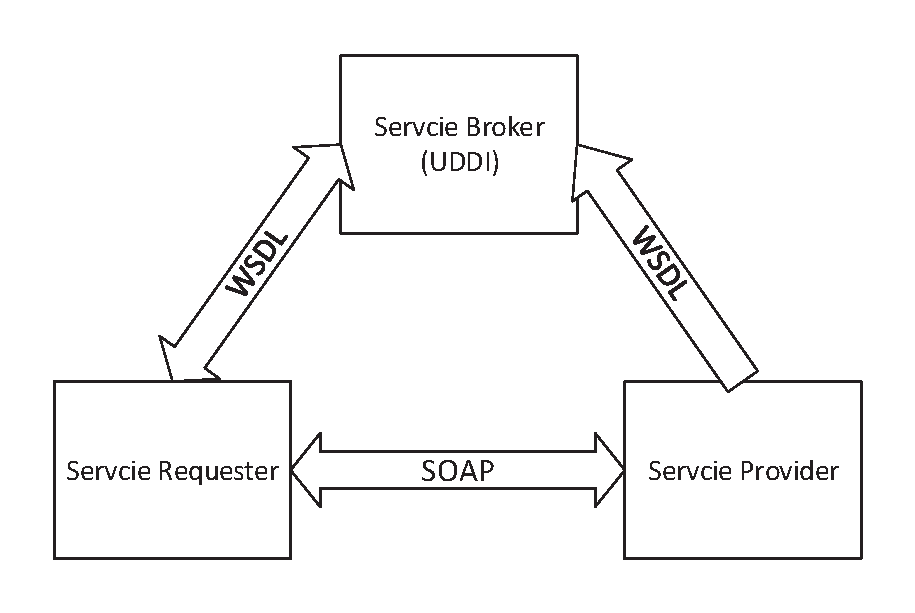
\includegraphics[width=0.6\textwidth]{web-service-arc}
  \caption{Web Service典型架构}
  \label{fig:web-service-arc}
\end{figure}

\subsubsection{REST服务架构概述}
REST(Representational state transfer)并不是特指具体一种通信协议,而是一种扩展服务设计的原则。随着近些年云服务的开展普及,REST在工业界得到了非常广泛的应用,如Amazon S3,微信公共账号接口等。与SOAP协议不同,REST需要直接利用HTTP协议作为传输协议,利用HTTP动词(GET,POST,PUT,DELETE)与URI的组合来定义REST的具体服务操作。

\subsubsection{存在的问题}

对于当前最普遍的两种Web服务架构即基于SOAP与REST普遍是现在HTTP协议之上。在SOAP中,包含服务请求与应答的XML报文直接封装在HTTP数据包之中。在REST中,资源直接通过HTTP的URI进行标记,通过HTTP动词对资源进行操作。HTTP协议已经成为事实上的网络瘦腰(narrw waist)。\cite{popa2010http}但以HTTP为承载的服务网络包含如下问题:HTTP为应用层协议,到物理层信号传输还要经过多层次的协议栈。而相关的经典协议栈如IP协议、以太网协议等兼顾通用性,未对事实上的瘦腰HTTP协议进行优化。例如HTTP协议无法阻止在底层网络层面阻止DDOS攻击,网络层面无法直接缓存数据包,需要服务提供商自建或租用CDN系统。REST架构的网络服务中,本质是面向资源,面向内容的状态控制变化的,客户端不需要关心服务或资源的具体位置。而当前底层最普遍的IP网络是面向连接的,在处理相同资源在不同的物理地址路由时,无法做到面向内容的优化路由。

\subsection{信息中心网络概述}

随着当今互联网数据分发流量的快速增长,TCP/IP架构在内容分发方面暴露出一些问题。因此信息中心网络(Information Centric Networking,ICN)作为一种新的网络架构设计原则被提出来。目前正在积极研究并开发的ICN网络项目有:DONA(Data-Oriented Network Architecture)\cite{koponen2007data},Named Data Networking(NDN)\cite{jacobson2009networking},Content-Centric Networking(CCN)\cite{jacobson2009networking},Publish-Subscribe Internet Routing Paradigm(PRISP)\cite{ain2009d2},Network of Information(NetInf)\cite{ahlgren2010second}等。虽然实现方式细节上各有不同,但是设计目标与架构特点相似。都是为了更有效率地获取与分发数据,并解决网络中断,流量洪泛等问题。网络通信通常由数据请求端驱动。网络包单位为命名数据对象(named data object,NDO)。\cite{ahlgren2012survey}ICN对于传统的TCP/IP架构网络的颠覆则是利用NDO来替代IP包作为新的网络瘦腰。

\section{研究内容及意义}
本论文主要研究利用信息中心网络的命名数据机制设计一种新的面向服务的网络架构,并对该架构进行原型实现与实验评估。具体研究内容为:
\begin{itemize}
\item 提出一种基于命名机制的服务网络协议设计,即命名服务网络协议;
\item 以命名服务网络协议为基础设计一套服务网络架构,包括服务发现,服务路由,安全验证,服务仲裁等组件
\item 提出一套服务网络比较框架,并与SOAP与REST的网络服务架构进行比较分析
\item 根据命名服务网络架构设计一种本地分布式计算系统方案
\end{itemize}
研究意义在于打破传统服务网络基于HTTP协议与TCP/IP面向连接的网络架构,充分利用信息中心网络的性质特点提出一种新的网络设计范式,并未未来服务网络实现提供一种可能方案。
\section{章节安排}
本论文公分7章,各章内容如下:

第一章介绍课题的背景与研究意义。

第二章介绍本文涉及到的服务网络包括Web Service以及信息中心网络的基本概况与研究进展。重点介绍命名数据网络的架构以及当前的开发动态。同时多种介绍基于信息中心网络的服务架构研究,分析比较各个研究特点并总结不足。

第三章介绍作者参与的基于命名数据网络存储软件的开发细节,并总结出基于命名数据网络服务开发的原则。

第四章介绍命名服务网络的协议与架构设计。

第五章进行命名服务网络的原型实现,并基于该原型进行实验评估。

第六章提出一种基于命名服务网络的本地分布式服务集群设计

第七章对前面所做工作进行总结并指出未来需要完善的工作,并对未来研究做出展望。



%%% Local Variables: 
%%% mode: latex
%%% TeX-master: t
%%% End: 

\chapter{相关工作}
\section{Web Service相关研究概述}
Web服务从广义上指基于网络的主机与主机之间互操作的软件系统。Web服务的主要特点在于提供轻量级的Web调用接口提供自足的(self-contained)松耦合的服务。狭义Web服务特指Web Service类似于W3C制定的基于SOAP协议的服务架构。该架构最基本的元素如引言所述的SOAP+WSDL+UDDI。关于Web Service架构的研究与应用开发在21世纪伊始比较热,而最近大与服务提供商更加倾向于使用形式上更加简单的REST接口。
\subsection{基于SOAP协议的Web Service}
\subsubsection{服务架构}
与工业界注重W3C及企业联盟注重标准制定与协议规范不同,学术界更加注重以通信协议为基础如何解决在资源动态变化的基础上解决日益复杂的应用需求。研究的问题主要包括Web数据集成、服务组合、访问控制、事件机制以及语义网(semantic web)相关研究。一个最基本的Web Service架构如图\ref{fig:web-service-arc-2}所示。

\begin{figure}[H]
  \centering
  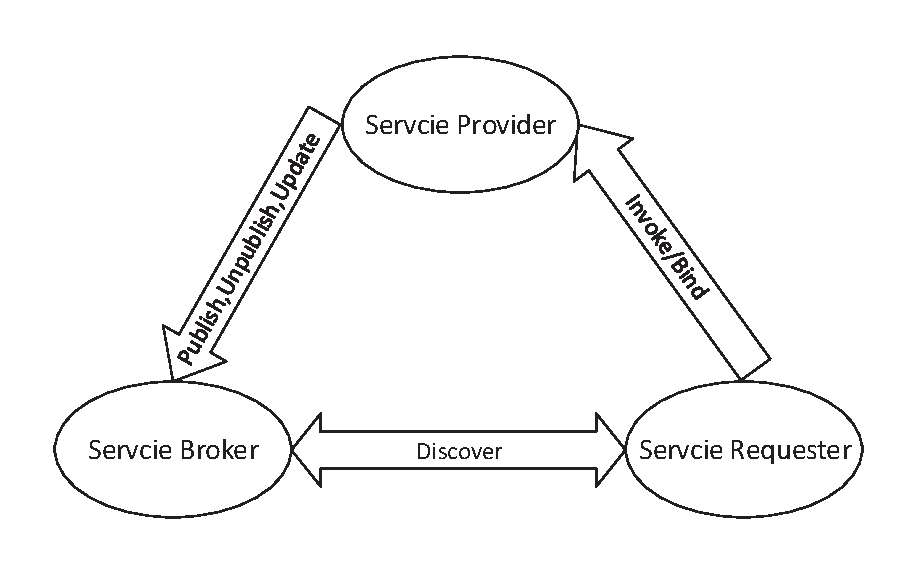
\includegraphics[width=0.6\textwidth]{web-service-arc-2}
  \caption{Web Service模型架构}
  \label{fig:web-service-arc-2}
\end{figure}

Bussler\cite{fensel2002web}指出由UDDI,WSDL和SOAP组成的协议栈无法实现真正可扩展的广域Web Service服务。实现可扩展的Web服务发现,选择,协调以及组合需要包含以下最基本的元素\cite{bussler2001b2b}:
\begin{itemize}
\item 文档类型(Document Types):文档类型为交换文档的基本语义。即文档类型定义了服务请求者与服务提供者数据交换的格式以及需要采取的语义(semantics)。
\item 语义(semantics):服务提供者与服务请求者确定相同的文档类型并保证传递信息语义的正确。因此需要语义词典来枚举文档元素所有可能的可用值。本体论(ontology)提供了一种对数据概念定义的一种手段,以保证对于数据概念解释的一致性。
\item 相关传输协议:服务请求双方需要约定好一致的通信协议。针对SOAP协议,底层协议可以为HTTP,SMTP,TCP,UDP或者JMS。
\item 信息交换序列:由于底层交换信息未必是可靠传输,可能发生报文重传与丢失现象,所以需要对交换报文添加序列号或消息确认以保证交换信息的完整性。
\item 流程:对于一个完整的服务而言,一次服务信息交换未必能够完成指定服务。例如一次购买行为,需要先将商品加入购物车,确定订单之后付款。之间至少需要三次服务请求双方的信息交换,并且顺序不能颠倒。所以服务双方需要确定一套服务协议流程。
\item 安全:安全性即服务最基本的需求,包括保证报文的私密性以及完整性。再次基础上还有服务与资源的访问控制等问题
\item 句法:即文档格式,如XML,JSON等
\item 服务配置:在各个相关服务端进行交互之前,可能服务主机的配置不相同,例如语义词典,服务流程等。当双方开始进行交互时,需要根据服务端进行特定配置。
\end{itemize}

文献\cite{fensel2002web}提出Web服务建模框架(Web Service Modeling Framework,WSMF)。WSMF旨在提出一套完全灵活并可扩展的Web服务架构。W3C也以WSMF框架为基础发布了一些列Web Service规范。\cite{WSMF-imp}WSMF架构。WSMF架构基于一下两个原则:元件,元素之间的强解耦性;强中介性,任何元素或服务之间可以通过扩展方式进行相互对话,强调元素与目标的的重用性及语义。WSMF的十字形架构如图\ref{fig:WSMF-arc}所示。图\ref{fig:WSMF-arc}采用文献\cite{WSMF-imp}的改进“十字形模型”。

\begin{figure}[H]
  \centering
  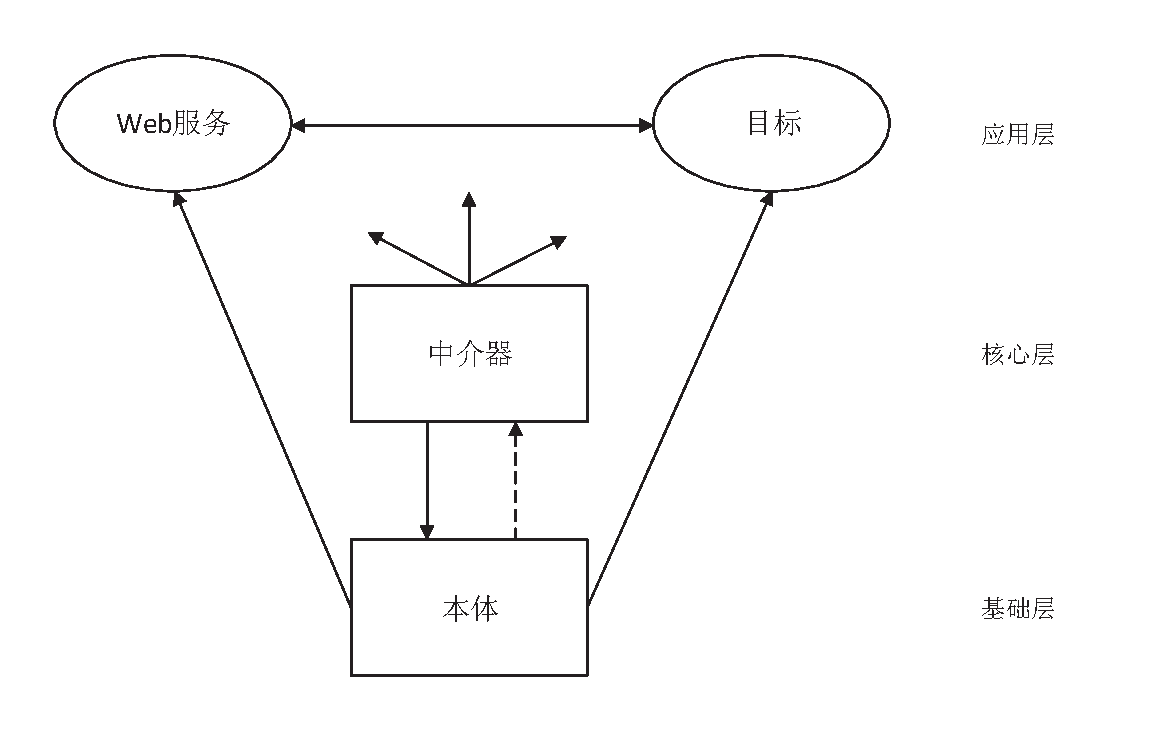
\includegraphics[width=0.7\textwidth]{WSMF-arc}
  \caption{WSMF顶层要素与相互关系}
  \label{fig:WSMF-arc}
\end{figure}

该模型中应用层为各种可被重用的任务集$\{\mathrm{WS}\mid\mathnormal{ws_{1}}, \mathnormal{ws_{2}}, \mathnormal{ws_{3}} \cdots \mathnormal{ws_{m}}\}$ 与$ \{\mathrm{G}\mid\mathnormal{g_{1}}, \mathnormal{g_{2}}, \mathnormal{g_{3}} \cdots \mathnormal{g_{n}}\}$。在具体实现相关应用时即为实现指定目标$\mathnormal{G_j}, \mathnormal{G_j}\subset\mathnormal{G}$而按一定流程重新组合$\mathnormal{W_i}, \mathnormal{W_i}\subset\mathnormal{W}$。

WSMF的核心为中介器,包括本体中介器,目标中介器,服务中介器,以及目标服务组着中介器。用来协调各个元素之间的组合关系。此外需要协调服务与服务之间包括传送协议,数据结构,信息格式的不同方言等问题。本体为WSMF架构的基础,对服务,目标,中介器进行描述和条件约束。

\subsubsection{服务发现}
在服务发现技术方面,服务发现是指服务请求者基于某单一既定目标查找选定需要的服务。工业界最常见的为UDDI服务,但依旧在更高的复杂性和信息组合自动化方面有所不足。当前Web服务发现的主要技术如表\ref{tab:web-service-discovery}所示。\cite{klein2001serching}

\begin{table}[htb]
  \centering
  \begin{minipage}[t]{0.8\linewidth}
  \caption{主流服务发现技术比较}
  \label{tab:web-service-discovery}
    \begin{tabular}{c	c	c	c}
      \toprule[1pt]
      \textbf{Service Discovery Technologies} & \textbf{Precision} & \textbf{Recall} & \textbf{Hardness} \\\midrule[0.5pt]
      Keyword Based & Low & High & Average\\
      Frame Based & High & Low & Average\\
      Deductive Retieval & High & High & Hard\\
      \bottomrule[1pt]
    \end{tabular}
  \end{minipage}
\end{table}

大多数检索方法是类似于基于UDDI的框架(Frame Based)方法。基于逻辑推导(Deductive Retieval)的方法由于服务在概念上与约束上非常难表述,所以实现难度最高。Mark Klein,Abraham Bernstein提出一套基于Ontology的服务发现架构,将服务描述通过语义网(Semantic Web)重新组织,提出了一套查询方式更加灵活,查询准确性更高的框架。\cite{klein2001serching}

\subsubsection{Web服务安全}
Web服务安全研究主要分为两个方面即,访问控制与数据安全。Web Service访问控制技术大体分为:
\begin{itemize}
\item 基于主机认证:基于访问主机请求中的网络认证信息(如hostname, IP等),缺点是无法控制区分同一主机的不同用户,信息也比较容易伪造。
\item 基本认证:基于辨识身份的用户名与密码,用户名与密码在基于HTTP的传输中保持为明文。
\item 基于SSL/TLS的身份证书:利用证书对传输信息进行加密或签名,是工业实现中相对可靠,并且主流的实现方式。而对证书的分发与信任模型(trust model)本身为密码工业的研究范围
\end{itemize}

WS-Security作为SOAP的扩展协议由OASIS于2002年提出。\cite{nadalin2002web}该协议旨在保证Web服务信息传输的加密型以及防止信息篡改。该协议支持多种安全信令包括X.509,Kerberos,以及 Security Assertion Markup Language(SAML),提供端到端的信息安全保护。

\subsection{基于REST的Web服务架构}
REST(表述性状态转移,Representational state transfer)不是指具体的某个协议,而是一种构建分布式可扩展web服务的最佳实践原则。REST通常通过HTTP协议来组织超媒体(Hypermedia)资源。

REST的主要设计原则为:
\begin{itemize}
\item 统一接口:通过HTTP动词(GET,POST,PUT,DELETE)对以URI标记的资源进行操作以代表创建,读取,更新,删除等操作
\item 自描述性:资源与其描述为松耦合,因此资源可以以不同的格式存在(XML,JPEG,PDF等)。客户端与服务端可以利用HTTP中对资源描述的元数据对资源进行操作
\item 无状态性:对于资源操作在服务端与客户端是无状态的。状态描述被显式的保存在超链接上。
\end{itemize}
以微信公共账号服务接口为例,采用REST风格的调用接口。通过服务号群发消息的接口如下:

\noindent
\fbox{
\parbox{0.9\textwidth}{
  \small{http请求方式: POST\\
  https://api.weixin.qq.com/cgi-bin/media/uploadnews?access\_token=ACCESS\_TOKEN}
 }
}

HTTP报文封装的POST的数据为JSON格式的一段文档。

一些组织也在进行基于REST的服务架构标准化工作,包括Open Mobile Alliance(OMA)以及IETF。OMA研究主要集中在基于Parlay-X(一种电话网络中Web Service的服务架构)REST接口研究与制定。\cite{alliancerestful}IETF也在制定基于REST的集中会议控制协议(Centralized Conferencing Manipulation Protocol,CCMP)\cite{barnes2009centralized}。

\section{信息中心网络相关研究概述}
\subsection{信息中心网络研究概述}
TCP/IP在早在20世纪70年代就被提了出来,当时网络的主要需求即为固定主机间端到端的可靠通信。且在简单IP层的瘦腰网络架构支持下,上层网络应用只要基于最简单的IP协议,即可在互联网上运行,所以大量的互联网创新应用随之而来。随着当今互联网越来越向数据分发的方向演进,以命名数据取代IP网络瘦腰的信息中心网络设计思想作为一种全新的架构被提出来。当前主要的ICN架构包括DONA,NDN,PRISP和NetInf。ICN设计主要考虑如下五个方面\cite{xylomenos2014survey}:

\begin{itemize}
\item 命名:在所有的ICN架构中,网络包的命名与主机地址无关。命名方式有两种,即扁平化或层次化的命名方式
\item 名字解析与数据路由:主要分为耦合和解耦两种方式。在耦合方式中,命名数据请求被转发到相应的主机后,数据沿着请求反向路径返回给数据请求者。在解耦方式中,数据应答的返回路径不做限制。
\item 缓存:缓存设计主要分为\textit{on-path}和\textit{off-path}两种。\textit{on-path}方式指的是数据被缓存在数据请求的转发路径上。\textit{off-path}缓存需要请求转发与路由系统支持,即缓存数据主机可以被当做正常的数据发布者
\item 移动:ICN天然地支持数据请求者的移动性,因为当请求链接失败之后,请求者可以在新的地点构建新的数据请求路径。而数据发布者的移动性支持较难,需要一定的路由机制重新更新请求路由转发表。
\item 安全:安全机制设计与数据命名方式直接相关。扁平的命名方式需要命名数据能够自验证,而结构化的命名方式则可以建立结构化的信任模型(trust model)。
\end{itemize}

\subsection{命名数据网络架构及研究进展}
本文中的命名服务网络设计主要基于ICN中的命名数据网络架构设计(Named Data Networking,NDN)。NDN架构在2009年由Van Jacobson等人提出。\cite{jacobson2009networking}NDN架构如图\ref{fig:IP-vs-NDN}所示。NDN的网络架构继承了IP架构的沙漏型瘦腰结构。由于瘦腰的简单性,上下层协议只要支持瘦腰协议即可进行大量创新,这个瘦腰架构也是互联网发展30年来的成功经验
。在NDN架构中利用命名数据包来取代以端主机地址标记的IP网络包。

\begin{figure}[H]
  \centering
  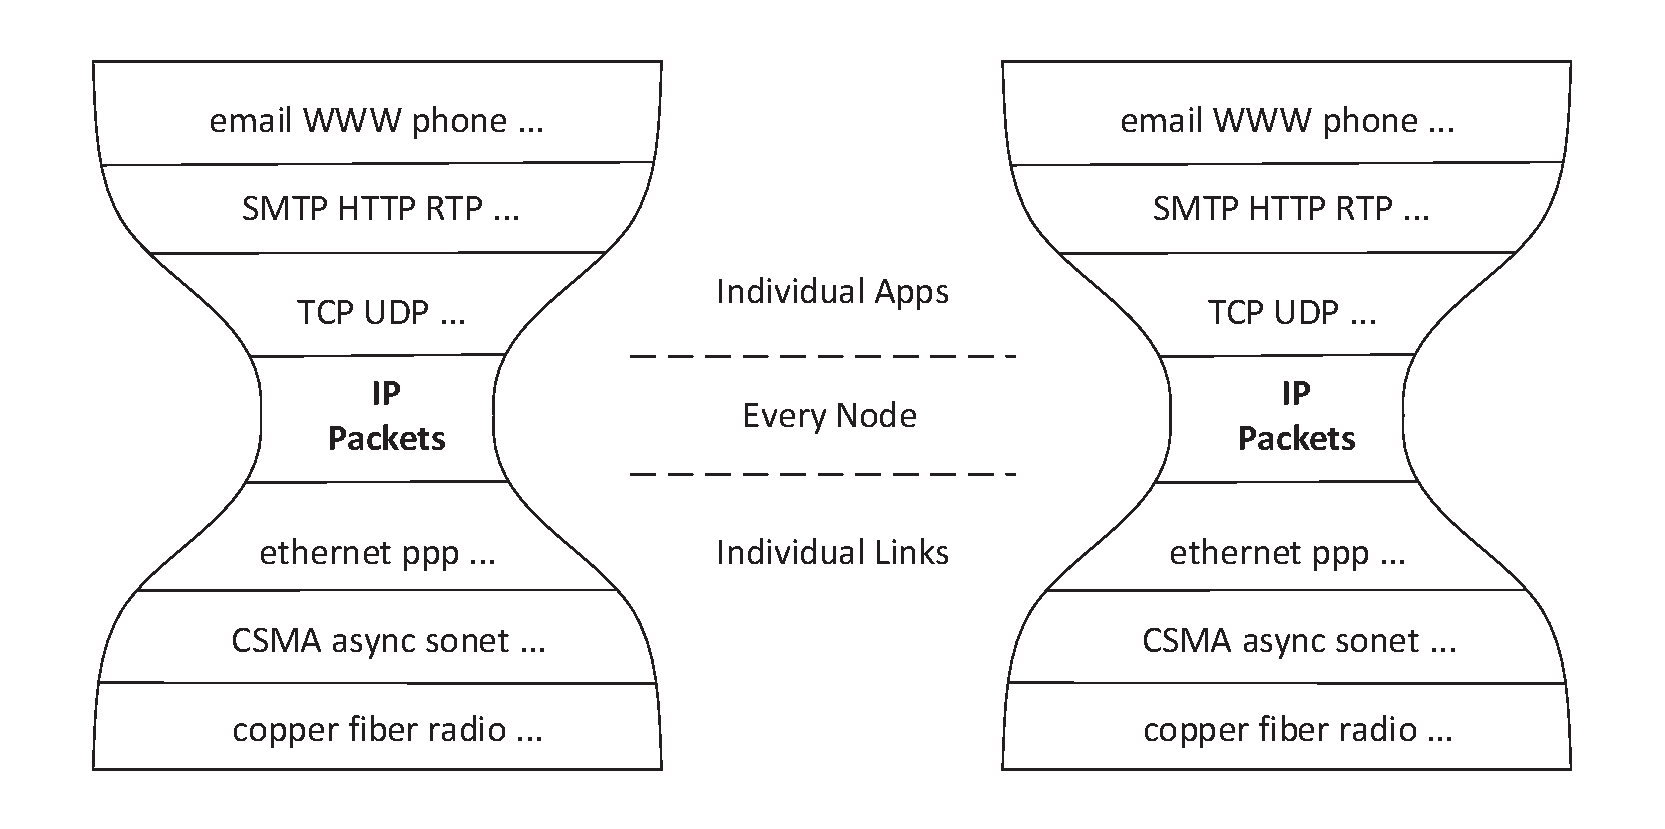
\includegraphics[width=0.9\textwidth]{IP-vs-NDN}
  \caption{IP与NDN架构对比}
  \label{fig:IP-vs-NDN}
\end{figure}

NDN的主要设计原则是:
\begin{itemize}
\item 命名:NDN采用结构化URI方式的命名。结构化的命名方式可以使路由更加具有扩展性,即可以采用名字前缀方式进行路由。命名方式不涉及网络上的信息如(IP地址)而是直接应用相关,即应用可以不依赖网络选择特定的命名方式。
\item 安全:安全特性在NDN架构的另一个基础。NDN架构采用以数据为中心的安全,及对每一个数据包单独进行签名。数据的安全性与数据在哪里存放解耦。
\item 名字解析与数据路由:名字解析不直接整合在NDN架构中,就像IP网络中DNS是独立的网络一样。NDN路由采用耦合方式,即数据会根据数据数据请求的转发路径反向转发。由于NDN采用前缀转发的方式与IP类似,所以NDN可以采用IP类似的BGP,IS-IS和OSPF转发协议。
\item 缓存:由于NDN采用耦合方式转发数据请求,数据可以被缓存在数据请求路径的中间节点上。而NDN与IP不同的是可以做到真正的网络层缓存。因为NDN数据包与IP数据包不同的是直接以应用数据名字命名,而不是以地址命名,所以在缓存中的数据可以被其他请求端重用。而由于NDN数据包的数据中心安全性,数据包缓存在网络中可以被加密也可以签名防止被篡改。
\item 智能数据平面:与IP不同,IP是一个无状态协议,路由器很难在IP的层面对路由状态进行监控。而NDN中的请求等待表(Pending Interest Table,PIT)记录了所转发数据请求的一些列转发状态信息。而抓发节点可以根据PIT所记录的软状态(soft state)构建智能的转发策略。
\end{itemize}

NDN数据包分两种,数据兴趣包(interest packet)与数据包(data packet),如图\ref{fig:NDN-packet}所示。兴趣包封装请求数据的名字以及一些其他选择条件。当兴趣包被转发到含有相应数据包的主机时,该节点可以返回相应的数据包。
\begin{figure}[H]
  \centering
  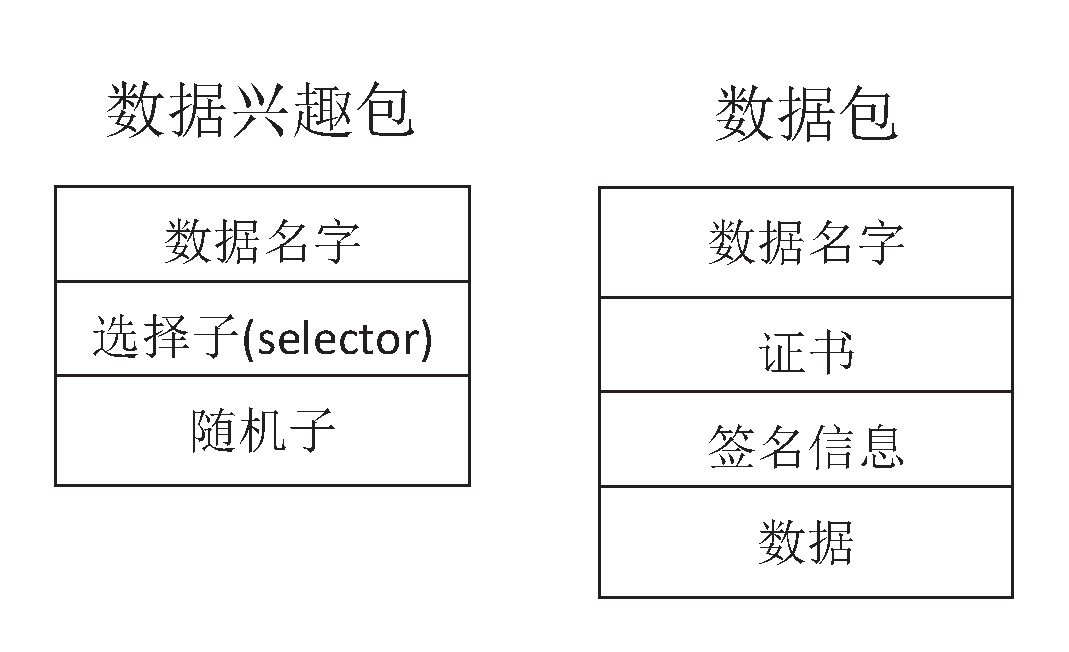
\includegraphics[width=0.7\textwidth]{NDN-packet}
  \caption{IP与NDN架构对比}
  \label{fig:NDN-packet}
\end{figure}

NDN协议处理架构主要是基于三个表即转发表(Forwarding Information Base,FIB),兴趣等待表(Pending Interest Table,PIT)与内容缓存(Content Store,CS)。FIB转发表类似于IP的转发表,用来存储名字前缀以及对应的转发接口。PIT表用来存储在本节点转发出去并且还没被相应的interest。CS表即内容缓存,用来缓存返回的数据包。

一个节点处理interest请求过程为,首先查找CS看是否有对应的数据包,如果有直接返回,如果没有则查找FIB表,看有没有转发的合适条目,如果存在则按照FIB规则转发,同时interest被存储在PIT中。当对应的请求包回到该节点时,一方面根据CS缓存策略对该数据包进行缓存,另一方面根据PIT表存储的interest信息返回该数据,并删除PIT表中的该条目。

\subsection{基于信息中心网络的服务网络相关研究}
ICN本质上是把传统网络中的\textit{where}模型转化为\textit{what}模型,网络直接处理的是应用数据的抽象。而一些研究在数据之上进一步地进行抽象,认为网络的本质是承载与连接服务。

文献\cite{nordstrom2012serval}提出一种服务中心网络协议栈(Serval)。通过ServiceID来标记应用网络包,通过FlowID用来标记当连接建立后的网络包。Serval协议栈中还增加了Service Table和Flow Table用来记录Service和Flow的网络状态,在Host端可以可以针对网络服务情况进行状态保持和只能决策。

文献\cite{braun2011service,braun2013service}中提出一种服务中心网络(Service-Centric Networking,SCN)架构以及一种基于NDN的服务中心网络实现。在沙漏架构中将NDN的命名数据包替换成服务对象。SCN修改Interest的结构使其能够封装服务请求参数。但整体来说SCN就是对NDN表述的重新抽象以及对流程的简单修改。

文献\cite{wu2014sofia}提出了一种基于ICN的面向服务信息网络架构(SOFIA)。而SOFIA的本质也是利用了NDN的命名、转发与缓存机制。此外在SOFIA中增加了Service Relay角色,相当于一种服务代理。服务请求者可以请求Service Relay在不同的网络环境中进行新的服务请求连接。这种机制有助于网络中multihoming,multicast以及mobility的实现。



%%% 其它部分
\backmatter

% 本科生要这几个索引,研究生不要。选择性留下。
\makeatletter
\ifthu@bachelor
  % 插图索引
  \listoffigures
  % 表格索引
  \listoftables
  % 公式索引
  %\listofequations
\fi
\makeatother


% 参考文献
\bibliographystyle{thubib}
\bibliography{ref/refs}


% 致谢
%%% Local Variables:
%%% mode: latex
%%% TeX-master: "../main"
%%% End:

\begin{ack}
  衷心感谢导师 xxx 教授和物理系 xxx 副教授对本人的精心指导。他们的言传身教将使
  我终生受益。

  在美国麻省理工学院化学系进行九个月的合作研究期间,承蒙 xxx 教授热心指导与帮助,不
  胜感激。感谢 xx 实验室主任 xx 教授,以及实验室全体老师和同学们的热情帮助和支
  持!本课题承蒙国家自然科学基金资助,特此致谢。

  感谢 \thuthesis,它的存在让我的论文写作轻松自在了许多,让我的论文格式规整漂亮了
  许多。
\end{ack}


% 附录
\begin{appendix}
%%% Local Variables: 
%%% mode: latex
%%% TeX-master: "../main"
%%% End: 

\chapter{外文资料原文}
\label{cha:engorg}
As one of the most widely used techniques in operations research, {\em
  mathematical programming} is defined as a means of maximizing a quantity known
as {\em objective function}, subject to a set of constraints represented by
equations and inequalities. Some known subtopics of mathematical programming are
linear programming, nonlinear programming, multiobjective programming, goal
programming, dynamic programming, and multilevel programming$^{[1]}$.

It is impossible to cover in a single chapter every concept of mathematical
programming. This chapter introduces only the basic concepts and techniques of
mathematical programming such that readers gain an understanding of them
throughout the book$^{[2,3]}$.


\section{Single-Objective Programming}
The general form of single-objective programming (SOP) is written
as follows,
\begin{equation}\tag*{(123)} % 如果附录中的公式不想让它出现在公式索引中,那就请
                             % 用 \tag*{xxxx}
\left\{\begin{array}{l}
\max \,\,f(x)\\[0.1 cm]
\mbox{subject to:} \\ [0.1 cm]
\qquad g_j(x)\le 0,\quad j=1,2,\cdots,p
\end{array}\right.
\end{equation}
which maximizes a real-valued function $f$ of
$x=(x_1,x_2,\cdots,x_n)$ subject to a set of constraints.

\newtheorem{mpdef}{Definition}[chapter]
\begin{mpdef}
In SOP, we call $x$ a decision vector, and
$x_1,x_2,\cdots,x_n$ decision variables. The function
$f$ is called the objective function. The set
\begin{equation}\tag*{(456)} % 这里同理,其它不再一一指定。
S=\left\{x\in\Re^n\bigm|g_j(x)\le 0,\,j=1,2,\cdots,p\right\}
\end{equation}
is called the feasible set. An element $x$ in $S$ is called a
feasible solution.
\end{mpdef}

\newtheorem{mpdefop}[mpdef]{Definition}
\begin{mpdefop}
A feasible solution $x^*$ is called the optimal
solution of SOP if and only if
\begin{equation}
f(x^*)\ge f(x)
\end{equation}
for any feasible solution $x$.
\end{mpdefop}

One of the outstanding contributions to mathematical programming was known as
the Kuhn-Tucker conditions\ref{eq:ktc}. In order to introduce them, let us give
some definitions. An inequality constraint $g_j(x)\le 0$ is said to be active at
a point $x^*$ if $g_j(x^*)=0$. A point $x^*$ satisfying $g_j(x^*)\le 0$ is said
to be regular if the gradient vectors $\nabla g_j(x)$ of all active constraints
are linearly independent.

Let $x^*$ be a regular point of the constraints of SOP and assume that all the
functions $f(x)$ and $g_j(x),j=1,2,\cdots,p$ are differentiable. If $x^*$ is a
local optimal solution, then there exist Lagrange multipliers
$\lambda_j,j=1,2,\cdots,p$ such that the following Kuhn-Tucker conditions hold,
\begin{equation}
\label{eq:ktc}
\left\{\begin{array}{l}
    \nabla f(x^*)-\sum\limits_{j=1}^p\lambda_j\nabla g_j(x^*)=0\\[0.3cm]
    \lambda_jg_j(x^*)=0,\quad j=1,2,\cdots,p\\[0.2cm]
    \lambda_j\ge 0,\quad j=1,2,\cdots,p.
\end{array}\right.
\end{equation}
If all the functions $f(x)$ and $g_j(x),j=1,2,\cdots,p$ are convex and
differentiable, and the point $x^*$ satisfies the Kuhn-Tucker conditions
(\ref{eq:ktc}), then it has been proved that the point $x^*$ is a global optimal
solution of SOP.

\subsection{Linear Programming} 
\label{sec:lp}

If the functions $f(x),g_j(x),j=1,2,\cdots,p$ are all linear, then SOP is called
a {\em linear programming}.

The feasible set of linear is always convex. A point $x$ is called an extreme
point of convex set $S$ if $x\in S$ and $x$ cannot be expressed as a convex
combination of two points in $S$. It has been shown that the optimal solution to
linear programming corresponds to an extreme point of its feasible set provided
that the feasible set $S$ is bounded. This fact is the basis of the {\em simplex
  algorithm} which was developed by Dantzig as a very efficient method for
solving linear programming.
\begin{table}[ht]
\centering
  \centering
  \caption*{Table~1\hskip1em This is an example for manually numbered table, which
    would not appear in the list of tables}
  \label{tab:badtabular2}
  \begin{tabular}[c]{|c|m{0.8in}|c|c|c|c|c|}\hline
    \multicolumn{2}{|c|}{Network Topology} & \# of nodes & 
    \multicolumn{3}{c|}{\# of clients} & Server \\\hline
    GT-ITM & Waxman Transit-Stub & 600 &
    \multirow{2}{2em}{2\%}& 
    \multirow{2}{2em}{10\%}& 
    \multirow{2}{2em}{50\%}& 
    \multirow{2}{1.2in}{Max. Connectivity}\\\cline{1-3}
    \multicolumn{2}{|c|}{Inet-2.1} & 6000 & & & &\\\hline
    \multirow{2}{1in}{Xue} & Rui  & Ni &\multicolumn{4}{c|}{\multirow{2}*{\thuthesis}}\\\cline{2-3}
    & \multicolumn{2}{c|}{ABCDEF} &\multicolumn{4}{c|}{} \\\hline
\end{tabular}  
\end{table}

Roughly speaking, the simplex algorithm examines only the extreme points of the
feasible set, rather than all feasible points. At first, the simplex algorithm
selects an extreme point as the initial point. The successive extreme point is
selected so as to improve the objective function value. The procedure is
repeated until no improvement in objective function value can be made. The last
extreme point is the optimal solution.

\subsection{Nonlinear Programming}

If at least one of the functions $f(x),g_j(x),j=1,2,\cdots,p$ is nonlinear, then
SOP is called a {\em nonlinear programming}.

A large number of classical optimization methods have been developed to treat
special-structural nonlinear programming based on the mathematical theory
concerned with analyzing the structure of problems.
\begin{figure}[h]
  \centering
  
\includegraphics[clip]{thu-lib-logo}
  \caption*{Figure~1\hskip1em This is an example for manually numbered figure,
    which would not appear in the list of figures}
  \label{tab:badfigure2}    
\end{figure}

Now we consider a nonlinear programming which is confronted solely with
maximizing a real-valued function with domain $\Re^n$.  Whether derivatives are
available or not, the usual strategy is first to select a point in $\Re^n$ which
is thought to be the most likely place where the maximum exists. If there is no
information available on which to base such a selection, a point is chosen at
random. From this first point an attempt is made to construct a sequence of
points, each of which yields an improved objective function value over its
predecessor. The next point to be added to the sequence is chosen by analyzing
the behavior of the function at the previous points. This construction continues
until some termination criterion is met. Methods based upon this strategy are
called {\em ascent methods}, which can be classified as {\em direct methods},
{\em gradient methods}, and {\em Hessian methods} according to the information
about the behavior of objective function $f$. Direct methods require only that
the function can be evaluated at each point. Gradient methods require the
evaluation of first derivatives of $f$. Hessian methods require the evaluation
of second derivatives. In fact, there is no superior method for all
problems. The efficiency of a method is very much dependent upon the objective
function.

\subsection{Integer Programming}

{\em Integer programming} is a special mathematical programming in which all of
the variables are assumed to be only integer values. When there are not only
integer variables but also conventional continuous variables, we call it {\em
  mixed integer programming}. If all the variables are assumed either 0 or 1,
then the problem is termed a {\em zero-one programming}. Although integer
programming can be solved by an {\em exhaustive enumeration} theoretically, it
is impractical to solve realistically sized integer programming problems. The
most successful algorithm so far found to solve integer programming is called
the {\em branch-and-bound enumeration} developed by Balas (1965) and Dakin
(1965). The other technique to integer programming is the {\em cutting plane
  method} developed by Gomory (1959).

\hfill\textit{Uncertain Programming\/}\quad(\textsl{BaoDing Liu, 2006.2})

\section*{References}
\noindent{\itshape NOTE: these references are only for demonstration, they are
  not real citations in the original text.}

\begin{enumerate}[{$[$}1{$]$}]
\item Donald E. Knuth. The \TeX book. Addison-Wesley, 1984. ISBN: 0-201-13448-9
\item Paul W. Abrahams, Karl Berry and Kathryn A. Hargreaves. \TeX\ for the
  Impatient. Addison-Wesley, 1990. ISBN: 0-201-51375-7
\item David Salomon. The advanced \TeX book.  New York : Springer, 1995. ISBN:0-387-94556-3
\end{enumerate}

\chapter{外文资料的调研阅读报告或书面翻译}
\section{单目标规划}
北冥有鱼,其名为鲲。鲲之大,不知其几千里也。化而为鸟,其名为鹏。鹏之背,不知其几
千里也。怒而飞,其翼若垂天之云。是鸟也,海运则将徙于南冥。南冥者,天池也。 
\begin{equation}\tag*{(123)}
 p(y|\mathbf{x}) = \frac{p(\mathbf{x},y)}{p(\mathbf{x})}=
\frac{p(\mathbf{x}|y)p(y)}{p(\mathbf{x})}
\end{equation}

吾生也有涯,而知也无涯。以有涯随无涯,殆已!已而为知者,殆而已矣!为善无近名,为
恶无近刑,缘督以为经,可以保身,可以全生,可以养亲,可以尽年。

\subsection{线性规划}
庖丁为文惠君解牛,手之所触,肩之所倚,足之所履,膝之所倚,砉然响然,奏刀騞然,莫
不中音,合于桑林之舞,乃中经首之会。
\begin{table}[ht]
\centering
  \centering
  \caption*{表~1\hskip1em 这是手动编号但不出现在索引中的一个表格例子}
  \label{tab:badtabular3}
  \begin{tabular}[c]{|c|m{0.8in}|c|c|c|c|c|}\hline
    \multicolumn{2}{|c|}{Network Topology} & \# of nodes & 
    \multicolumn{3}{c|}{\# of clients} & Server \\\hline
    GT-ITM & Waxman Transit-Stub & 600 &
    \multirow{2}{2em}{2\%}& 
    \multirow{2}{2em}{10\%}& 
    \multirow{2}{2em}{50\%}& 
    \multirow{2}{1.2in}{Max. Connectivity}\\\cline{1-3}
    \multicolumn{2}{|c|}{Inet-2.1} & 6000 & & & &\\\hline
    \multirow{2}{1in}{Xue} & Rui  & Ni &\multicolumn{4}{c|}{\multirow{2}*{\thuthesis}}\\\cline{2-3}
    & \multicolumn{2}{c|}{ABCDEF} &\multicolumn{4}{c|}{} \\\hline
\end{tabular}  
\end{table}

文惠君曰:“嘻,善哉!技盖至此乎?”庖丁释刀对曰:“臣之所好者道也,进乎技矣。始臣之
解牛之时,所见无非全牛者;三年之后,未尝见全牛也;方今之时,臣以神遇而不以目视,
官知止而神欲行。依乎天理,批大郤,导大窾,因其固然。技经肯綮之未尝,而况大坬乎!
良庖岁更刀,割也;族庖月更刀,折也;今臣之刀十九年矣,所解数千牛矣,而刀刃若新发
于硎。彼节者有间而刀刃者无厚,以无厚入有间,恢恢乎其于游刃必有余地矣。是以十九年
而刀刃若新发于硎。虽然,每至于族,吾见其难为,怵然为戒,视为止,行为迟,动刀甚微,
謋然已解,如土委地。提刀而立,为之而四顾,为之踌躇满志,善刀而藏之。”

文惠君曰:“善哉!吾闻庖丁之言,得养生焉。”


\subsection{非线性规划}
孔子与柳下季为友,柳下季之弟名曰盗跖。盗跖从卒九千人,横行天下,侵暴诸侯。穴室枢
户,驱人牛马,取人妇女。贪得忘亲,不顾父母兄弟,不祭先祖。所过之邑,大国守城,小
国入保,万民苦之。孔子谓柳下季曰:“夫为人父者,必能诏其子;为人兄者,必能教其弟。
若父不能诏其子,兄不能教其弟,则无贵父子兄弟之亲矣。今先生,世之才士也,弟为盗
跖,为天下害,而弗能教也,丘窃为先生羞之。丘请为先生往说之。”
\begin{figure}[h]
  \centering
  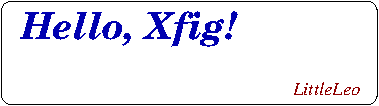
\includegraphics{hello}
  \caption*{图~1\hskip1em 这是手动编号但不出现索引中的图片的例子}
  \label{tab:badfigure3}    
\end{figure}

柳下季曰:“先生言为人父者必能诏其子,为人兄者必能教其弟,若子不听父之诏,弟不受
兄之教,虽今先生之辩,将奈之何哉?且跖之为人也,心如涌泉,意如飘风,强足以距敌,
辩足以饰非。顺其心则喜,逆其心则怒,易辱人以言。先生必无往。”

孔子不听,颜回为驭,子贡为右,往见盗跖。

\subsection{整数规划}
盗跖乃方休卒徒大山之阳,脍人肝而餔之。孔子下车而前,见谒者曰:“鲁人孔丘,闻将军
高义,敬再拜谒者。”谒者入通。盗跖闻之大怒,目如明星,发上指冠,曰:“此夫鲁国之
巧伪人孔丘非邪?为我告之:尔作言造语,妄称文、武,冠枝木之冠,带死牛之胁,多辞缪
说,不耕而食,不织而衣,摇唇鼓舌,擅生是非,以迷天下之主,使天下学士不反其本,妄
作孝弟,而侥幸于封侯富贵者也。子之罪大极重,疾走归!不然,我将以子肝益昼餔之膳。”


\chapter{其它附录}
前面两个附录主要是给本科生做例子。其它附录的内容可以放到这里,当然如果你愿意,可
以把这部分也放到独立的文件中,然后将其 \verb|\input| 到主文件中。
\end{appendix}

% 个人简历
\begin{resume}

  \resumeitem{个人简历}

  xxxx 年 xx 月 xx 日出生于 xx 省 xx 县。
  
  xxxx 年 9 月考入 xx 大学 xx 系 xx 专业,xxxx 年 7 月本科毕业并获得 xx 学士学位。
  
  xxxx 年 9 月免试进入 xx 大学 xx 系攻读 xx 学位至今。

  \resumeitem{发表的学术论文} % 发表的和录用的合在一起

  \begin{enumerate}[{[}1{]}]
  \item Yang Y, Ren T L, Zhang L T, et al. Miniature microphone with silicon-
    based ferroelectric thin films. Integrated Ferroelectrics, 2003,
    52:229-235. (SCI 收录, 检索号:758FZ.)
  \item 杨轶, 张宁欣, 任天令, 等. 硅基铁电微声学器件中薄膜残余应力的研究. 中国机
    械工程, 2005, 16(14):1289-1291. (EI 收录, 检索号:0534931 2907.)
  \item 杨轶, 张宁欣, 任天令, 等. 集成铁电器件中的关键工艺研究. 仪器仪表学报,
    2003, 24(S4):192-193. (EI 源刊.)
  \item Yang Y, Ren T L, Zhu Y P, et al. PMUTs for handwriting recognition. In
    press. (已被 Integrated Ferroelectrics 录用. SCI 源刊.)
  \item Wu X M, Yang Y, Cai J, et al. Measurements of ferroelectric MEMS
    microphones. Integrated Ferroelectrics, 2005, 69:417-429. (SCI 收录, 检索号
    :896KM.)
  \item 贾泽, 杨轶, 陈兢, 等. 用于压电和电容微麦克风的体硅腐蚀相关研究. 压电与声
    光, 2006, 28(1):117-119. (EI 收录, 检索号:06129773469.)
  \item 伍晓明, 杨轶, 张宁欣, 等. 基于MEMS技术的集成铁电硅微麦克风. 中国集成电路, 
    2003, 53:59-61.
  \end{enumerate}

  \resumeitem{研究成果} % 有就写,没有就删除
  \begin{enumerate}[{[}1{]}]
  \item 任天令, 杨轶, 朱一平, 等. 硅基铁电微声学传感器畴极化区域控制和电极连接的
    方法: 中国, CN1602118A. (中国专利公开号.)
  \item Ren T L, Yang Y, Zhu Y P, et al. Piezoelectric micro acoustic sensor
    based on ferroelectric materials: USA, No.11/215, 102. (美国发明专利申请号.)
  \end{enumerate}
\end{resume}

\end{document}
